\documentclass{beamer}

%%%%%%%%%%%%%%%%%%%%%%%%%%%%%%%%%%%%%%%%%%%%%%%%%%%%%%%%%%%%%%%%%%%%%%%%%%%%%%%%
% Packages
%%%%%%%%%%%%%%%%%%%%%%%%%%%%%%%%%%%%%%%%%%%%%%%%%%%%%%%%%%%%%%%%%%%%%%%%%%%%%%%%

% Warn about commands, classes and packages that are outdated and superseded.
% Orthodox checks for pitfalls that are not technically incorrect.
%\usepackage[l2tabu,orthodox,abort]{nag}

% For font and input encoding.
\usepackage[utf8]{inputenc}
%\usepackage[T1]{fontenc}

% Pretty much all of the ams maths packages.
\usepackage{amsmath,amsthm,amssymb,amsfonts}

% Allows inclusion of graphics easily and "configurably".
\usepackage{graphicx}

% Typesets URLs sensibly --- with a TrueType font, hyperlinked in PDFs, and not
% breaking across lines.
\usepackage{url}

% Count the number of used registers (counter, dimen, skip, muskip, box, token,
% input, output, math families, languages, insertions). Also time the amount of
% time required for LaTeX compilation.
\usepackage[timer,left]{regstats}

% For greater control over customising lists.
\usepackage{enumitem}

% The listings package is a source code printer for LaTeX. You can typeset stand
% alone files as well as listings with an environment similar to verbatim as
% well as you can print code snippets using a command similar to \verb.
\usepackage{listings}

% This package implements high-level interface commands for class file writers
% which allows the separation of formatting commands (typically instances of
% so-called `templates') and their arguments from the signature of
% document-level commands.
\usepackage{xparse}

% This package allows verbatim text to be typeset in bold.
\usepackage{alltt}
\renewcommand{\ttdefault}{txtt}

% This style option improves the interface for defining floating objects such
% as figures and tables in LaTeX. It adds the notion of a `float style' that
% governs appearance of floats. New kinds of floats may be defined using a
% \newfloat command analogous to \newtheorem. This style option also
% incorporates the functionality of David Carlisle's style option here, giving
% floating environments a [H] option which means `PUT IT HERE' (as opposed to
% the standard [h] option which means `You may put it here if you like').
\usepackage{float}

% This is the style file for the gnuplot PGF/TikZ terminal. It is associated
% with the 'gnuplot.lua' script.
\usepackage{gnuplot-lua-tikz}

% The caption package provides many ways to customise the captions in floating
% environments such figure and table.
\usepackage{caption}

% This package supports typesetting of sub-captions (by using the the
% sub-caption feature of the caption package).
\usepackage{subcaption}

% A new environment, tabularx, is defined, which takes the same arguments as
% tabular*, but modifies the widths of certain columns, rather than the inter
% column space, to set a table with the requested total width. The columns that
% may stretch are marked with the new token X in the preamble argument.
% NOTE: Requires the array package
\usepackage{array}
\usepackage{tabularx}

% This package reimplements the LATEX verbatim and verbatim* environments. In
% addition it provides a comment environment that skips any commands or text
% between \begin{comment} and the next \end{comment}. It also defines the
% command verbatim to input a whole file verbatim.
\usepackage{verbatim}

\usepackage[noline,ruled]{algorithm2e}
\usepackage{pgfplots}
\usepackage{tikz}
\usetikzlibrary{positioning,shapes,shadows,arrows}

% For animations
\usepackage{multimedia}

% My custom packages.
\usepackage{escape,citationneeded,pieplots,persons,pgf-pie}

%%%%%%%%%%%%%%%%%%%%%%%%%%%%%%%%%%%%%%%%%%%%%%%%%%%%%%%%%%%%%%%%%%%%%%%%%%%%%%%%
% Beamer configuration.
%%%%%%%%%%%%%%%%%%%%%%%%%%%%%%%%%%%%%%%%%%%%%%%%%%%%%%%%%%%%%%%%%%%%%%%%%%%%%%%%
% Presentation mode
\mode<presentation>

% No navigation symbols
\beamertemplatenavigationsymbolsempty

% Load a theme
\usetheme{Warsaw}
\useoutertheme[footline=authortitle]{miniframes}

\setbeamerfont{caption}{size=\scriptsize}

% Show notes
%\setbeameroption{show notes}

%%%%%%%%%%%%%%%%%%%%%%%%%%%%%%%%%%%%%%%%%%%%%%%%%%%%%%%%%%%%%%%%%%%%%%%%%%%%%%%%
% Custom colours
%%%%%%%%%%%%%%%%%%%%%%%%%%%%%%%%%%%%%%%%%%%%%%%%%%%%%%%%%%%%%%%%%%%%%%%%%%%%%%%%
\definecolor{darkGreen}{rgb}{0,0.6,0}
\definecolor{gray}{rgb}{0.5,0.5,0.5}
\definecolor{mauve}{rgb}{0.58,0,0.82}
\definecolor{brightGreen}{rgb}{0,1,0}

%%%%%%%%%%%%%%%%%%%%%%%%%%%%%%%%%%%%%%%%%%%%%%%%%%%%%%%%%%%%%%%%%%%%%%%%%%%%%%%%
% Source code formatting
%%%%%%%%%%%%%%%%%%%%%%%%%%%%%%%%%%%%%%%%%%%%%%%%%%%%%%%%%%%%%%%%%%%%%%%%%%%%%%%%
% Default settings
\lstset{
    basicstyle=\ttfamily,           % font
                                    %
    title=\lstname,                 % show the filename of files included with \lstinputlisting
    captionpos=b,                   % sets the caption-position to bottom
    backgroundcolor=\color{white},  % choose the background color
                                    %
    numbers=left,                   % where to put the line-numbers
    numberstyle=\tiny\color{gray},  % the style that is used for the line-numbers
    stepnumber=1,                   % the step between two line-numbers
    numbersep=5pt,                  % how far the line-numbers are from the code
                                    %
    showspaces=false,               % show spaces adding particular underscores
    showstringspaces=false,         % underline spaces within strings
    showtabs=false,                 % show tabs within strings adding particular underscores
    tabsize=4,                      % sets default tabsize
    breaklines=true,                % sets automatic line breaking
    breakatwhitespace=false,        % sets if automatic breaks should only happen at whitespace
                                    %
    keywordstyle=\color{blue},      % keyword style
    commentstyle=\color{darkGreen}, % comment style
    stringstyle=\color{mauve},      % string literal style
    escapeinside={\%*}{*)},         % if you want to add a comment within your code
    morekeywords={*,...}            % if you want to add more keywords to the set
}
\lstloadlanguages{C,Matlab}

%%%%%%%%%%%%%%%%%%%%%%%%%%%%%%%%%%%%%%%%%%%%%%%%%%%%%%%%%%%%%%%%%%%%%%%%%%%%%%%%
% Variables (to save retyping and reformatting these throughout the document).
%%%%%%%%%%%%%%%%%%%%%%%%%%%%%%%%%%%%%%%%%%%%%%%%%%%%%%%%%%%%%%%%%%%%%%%%%%%%%%%%
%%%%%%%%%%%%%%%%%%%%%%%%%%%%%%%%%%%%%%%%%%%%%%%%%%%%%%%%%%%%%%%%%%%%%%%%%%%%%%%%
% Variables (to save retyping and reformatting these throughout the document).
%%%%%%%%%%%%%%%%%%%%%%%%%%%%%%%%%%%%%%%%%%%%%%%%%%%%%%%%%%%%%%%%%%%%%%%%%%%%%%%%
\usepackage{definevariable} % for \defineVariable
\usepackage{persons} % for \definePerson, \getPerson, \formatPerson

\defineVariable\thesis{}{Thesis}
\defineVariable\thesisTitle{\textsc}{Implementation of Random Projection Algorithms Using an FPGA}
\defineVariable\thesisDate{}{2012}
\defineVariable\studentName{\formatPerson}{\getPerson*{Spence}}
\defineVariable\supervisorName{\formatPerson}{\getPerson*{Leong}}

\defineVariable\degreeName{}{Bachelor of Engineering (Computer)}
\defineVariable\schoolName{}{School of Electrical Engineering}
\defineVariable\studentID{}{308216350}
\defineVariable\universityName{}{The University of Sydney}
\defineVariable\uosAssessment{}{\thesis}
\defineVariable\uosCode{}{ELEC4712/ELEC4713}

\urldef{\gitRepoHTTP}\url{https://github.com/joshuaspence/ThesisCode.git}
\urldef{\gitRepoSSH}\url{git@github.com:joshuaspence/ThesisCode.git}

% People
\definePerson{Chawla}{Sanjay Chawla}
\definePerson{Frechtling}{Michael Frechtling}
\definePerson{Heinrichs}{Amelia Heinrichs}
\definePerson{Khoa}{Nguyen Lu Dang Khoa}
\definePerson{Leong}{Philip Leong}
\definePerson{Spence}{Joshua Spence}

% PDF metadata
\newcommand*\pdfmetadata{%
    pdfauthor={Joshua Spence},
    pdftitle={Implementation of Random Projection Algorithms Using an FPGA},
    pdfsubject={},
    pdfkeywords={commute time,anomaly detection,FPGA},
    pdfdisplaydoctitle={true}
}

% Copyrights and trademarks
\newcommand\ARM{ARM\textsuperscript{\textregistered}}
\newcommand\Cortex{Cortex\textsuperscript{\texttrademark}}
\newcommand\IntelXeon{Intel\textsuperscript{\textregistered} Xeon\textsuperscript{\textregistered}}
\newcommand\IntelCoreiSeven{Intel\textsuperscript{\textregistered} Core\textsuperscript{\texttrademark} i7}
\newcommand\AutoESL{\software{Xilinx\textsuperscript{\textregistered} AutoESL}}
\newcommand\ModelSim{\software{Altera\textsuperscript{\textregistered} ModelSim}}
\newcommand\Xilinx{Xilinx\textsuperscript{\textregistered}}

%%%%%%%%%%%%%%%%%%%%%%%%%%%%%%%%%%%%%%%%%%%%%%%%%%%%%%%%%%%%%%%%%%%%%%%%%%%%%%%%
% Custom commands
%%%%%%%%%%%%%%%%%%%%%%%%%%%%%%%%%%%%%%%%%%%%%%%%%%%%%%%%%%%%%%%%%%%%%%%%%%%%%%%%

%===============================================================================
% Format a block size profiling plot.
%-------------------------------------------------------------------------------
% \blockSizeProfilingPlot{DATASET}
%===============================================================================
\makeatletter
\newcommand\blockSizeProfilingPlot[1]{%
    \makebox[\textwidth][c]{%
        \resizebox{!}{0.85\textheight}{%
            \input{plots/block_size/#1}%
        }%
    }%
}
\makeatother

%===============================================================================
% Format a profiling plot.
%-------------------------------------------------------------------------------
% \profilingPlots{DATASET1}{DATASET2}{DATASET3}
%===============================================================================
\makeatletter
\newcommand\profilingPlots[3]{%
    \begin{columns}[c]%
        \column{0.33\textwidth}%
        \begin{figure}%
            \includegraphics[width=0.9\textwidth]{pca/#1}\\%
            \resizebox{0.7\textwidth}{!}{\input{plots/c/#1}}%
            \caption{\escape{#1}}%
        \end{figure}%
        %
        \column{0.33\textwidth}%
        \begin{figure}%
            \includegraphics[width=0.9\textwidth]{pca/#2}\\%
            \resizebox{0.7\textwidth}{!}{\input{plots/c/#2}}%
            \caption{\escape{#2}}%
        \end{figure}%
        %
        \column{0.33\textwidth}%
        \begin{figure}%
            \includegraphics[width=0.9\textwidth]{pca/#3}\\%
            \resizebox{0.7\textwidth}{!}{\input{plots/c/#3}}%
            \caption{\escape{#3}}%
        \end{figure}%
    \end{columns}%
    \vfill
    \makebox[\textwidth][c]{%
        \resizebox{!}{0.15\textheight}{%
            \pielegend[bound,color={yellow!60,blue!60,white!60,orange!60}]{
1/\escape{top_n_outlier_pruning_block},
1/\escape{distance_squared},
1/\escape{Other},
1/\escape{add_neighbour}
}
%
        }%
    }%
}
\makeatother

%%%%%%%%%%%%%%%%%%%%%%%%%%%%%%%%%%%%%%%%%%%%%%%%%%%%%%%%%%%%%%%%%%%%%%%%%%%%%%%%
% Custom formatting commands
%%%%%%%%%%%%%%%%%%%%%%%%%%%%%%%%%%%%%%%%%%%%%%%%%%%%%%%%%%%%%%%%%%%%%%%%%%%%%%%%

%===============================================================================
% Format the name of an algorithm.
%-------------------------------------------------------------------------------
% \algm{}
%===============================================================================
\newcommand\algm[1]{\emph{#1}}

%===============================================================================
% Format the name of a command line command. Also allows words to be broken over
% multiple lines
%
% See: http://jevopi.blogspot.com.au/2010/04/latex-lstinline-and-hyphenations.html
%-------------------------------------------------------------------------------
% \command{CMD}
%===============================================================================
\newcommand\command[1]{\lstinline[breaklines,literate={\_}{}{0\discretionary{\_}{}{\_}}]`#1`}

%===============================================================================
% Format the name of a data set.
%-------------------------------------------------------------------------------
% \dataset{DATASET}
%===============================================================================
\newcommand\dataset[1]{`\escape{#1}'}

%===============================================================================
% Format a computer host name.
%-------------------------------------------------------------------------------
% \hostname{HOSTNAME}
%===============================================================================
\newcommand\hostname[1]{\emph{#1}}

%===============================================================================
% Format the name of a programming language.
%-------------------------------------------------------------------------------
% \progLang{LANG}
%===============================================================================
\newcommand\progLang[1]{\lstinline`#1`}

%===============================================================================
% Format the name of a software package.
%-------------------------------------------------------------------------------
% \software{NAME}[CMD]
%===============================================================================
\NewDocumentCommand\software{om}{``#2''\IfNoValueTF{#1}{}{\space(\command{#1})}}

%%%%%%%%%%%%%%%%%%%%%%%%%%%%%%%%%%%%%%%%%%%%%%%%%%%%%%%%%%%%%%%%%%%%%%%%%%%%%%%%
% Graphics directory
%%%%%%%%%%%%%%%%%%%%%%%%%%%%%%%%%%%%%%%%%%%%%%%%%%%%%%%%%%%%%%%%%%%%%%%%%%%%%%%%
\graphicspath{{../img/}}

%%%%%%%%%%%%%%%%%%%%%%%%%%%%%%%%%%%%%%%%%%%%%%%%%%%%%%%%%%%%%%%%%%%%%%%%%%%%%%%%
% Title page options
%%%%%%%%%%%%%%%%%%%%%%%%%%%%%%%%%%%%%%%%%%%%%%%%%%%%%%%%%%%%%%%%%%%%%%%%%%%%%%%%
\title{\texorpdfstring{\thesisTitle*{}}{\thesisTitle}}
\author[\studentName*{}]{\texorpdfstring{\studentName*{}\\{\tiny{Supervisor: \supervisorName*{}}}}{\studentName*{}}}
\date{\thesisDate*{}}
\institute{\universityName*{}}
\titlegraphic{
\includegraphics[width=0.25\textwidth]{sydney_uni_coat_of_arms}}

%%%%%%%%%%%%%%%%%%%%%%%%%%%%%%%%%%%%%%%%%%%%%%%%%%%%%%%%%%%%%%%%%%%%%%%%%%%%%%%%
% Bibliography
%%%%%%%%%%%%%%%%%%%%%%%%%%%%%%%%%%%%%%%%%%%%%%%%%%%%%%%%%%%%%%%%%%%%%%%%%%%%%%%%
\usepackage[backend=bibtex,language=australian]{biblatex} % use biblatex instead of bibtex
\bibliography{thesis}

%%%%%%%%%%%%%%%%%%%%%%%%%%%%%%%%%%%%%%%%%%%%%%%%%%%%%%%%%%%%%%%%%%%%%%%%%%%%%%%%
%                               END OF PREAMBLE                                %
%%%%%%%%%%%%%%%%%%%%%%%%%%%%%%%%%%%%%%%%%%%%%%%%%%%%%%%%%%%%%%%%%%%%%%%%%%%%%%%%
\begin{document}

%%%%%%%%%%%%%%%%%%%%%%%%%%%%%%%%%%%%%%%%%%%%%%%%%%%%%%%%%%%%%%%%%%%%%%%%%%%%%%%%
% Title Page
%%%%%%%%%%%%%%%%%%%%%%%%%%%%%%%%%%%%%%%%%%%%%%%%%%%%%%%%%%%%%%%%%%%%%%%%%%%%%%%%
\begin{frame}[shrink]
    \titlepage
    % Title
    % Author names
    % University logo
\end{frame}

%%%%%%%%%%%%%%%%%%%%%%%%%%%%%%%%%%%%%%%%%%%%%%%%%%%%%%%%%%%%%%%%%%%%%%%%%%%%%%%%
% Introduction
%%%%%%%%%%%%%%%%%%%%%%%%%%%%%%%%%%%%%%%%%%%%%%%%%%%%%%%%%%%%%%%%%%%%%%%%%%%%%%%%
\section{Introduction}
\label{introduction}
%%%%%%%%%%%%%%%%%%%%%%%%%%%%%%%%%%%%%%%%%%%%%%%%%%%%%%%%%%%%%%%%%%%%%%%%%%%%%%%%
% Overview
%%%%%%%%%%%%%%%%%%%%%%%%%%%%%%%%%%%%%%%%%%%%%%%%%%%%%%%%%%%%%%%%%%%%%%%%%%%%%%%%
% Briefly tell the audience what you are going to cover.
\subsection{Overview}
\begin{frame}[label=overview]{Overview}
    \begin{itemize}
        \item Anomaly detection algorithm using commute time and Eigenspace
            approximation.
        \item Software-hardware coprocessing.
        \item Hardware implementation.
        \item A bullet on FPGAs.
        \item Reconfigurable computing is the application of FPGAs to computing problems.
    \end{itemize}
\end{frame}

%%%%%%%%%%%%%%%%%%%%%%%%%%%%%%%%%%%%%%%%%%%%%%%%%%%%%%%%%%%%%%%%%%%%%%%%%%%%%%%%
% Motivation
%%%%%%%%%%%%%%%%%%%%%%%%%%%%%%%%%%%%%%%%%%%%%%%%%%%%%%%%%%%%%%%%%%%%%%%%%%%%%%%%
% Briefly tell the audience why you are doing your research. Sell your audience
% on why your topic is important and of interest to them.
\subsection{Motivation}
\begin{frame}[label=motivation]{Motivation}
    \begin{itemize}
        \item The amount of data being collected and stored is continually
            increasing.
        \item Anomaly detection is an important technique which can be applied
            to a wide range of applications.
    \end{itemize}
\end{frame}

\begin{frame}[label=applications]{Applications}
    \begin{itemize}
        \item Stock market analysis
        \item Network intrusion detection
        \item Image comparison
        \item Fraud detection
        \item Data cleaning
        \item Detecting employers with poor injury histories
    \end{itemize}
\end{frame}

%%%%%%%%%%%%%%%%%%%%%%%%%%%%%%%%%%%%%%%%%%%%%%%%%%%%%%%%%%%%%%%%%%%%%%%%%%%%%%%%
% Aims
%%%%%%%%%%%%%%%%%%%%%%%%%%%%%%%%%%%%%%%%%%%%%%%%%%%%%%%%%%%%%%%%%%%%%%%%%%%%%%%%
% This section should be short and memorable.
\subsection{Aims}
\begin{frame}[label=aims]{Aims}
    The aim of this \thesis{} is to \emph{investigate the performance benefits}
    that can be obtained by \emph{applying reconfigurable computing design
    principles} to an \emph{anomaly detection algorithm} using commute time and
    Eigenspace sampling.
\end{frame}

%%%%%%%%%%%%%%%%%%%%%%%%%%%%%%%%%%%%%%%%%%%%%%%%%%%%%%%%%%%%%%%%%%%%%%%%%%%%%%%%
% Contributions
%%%%%%%%%%%%%%%%%%%%%%%%%%%%%%%%%%%%%%%%%%%%%%%%%%%%%%%%%%%%%%%%%%%%%%%%%%%%%%%%
% What I contributed towards this research area.
\subsection{Contributions}
\begin{frame}[label=contributions]{Contributions}
    \begin{enumerate}
        \item Quantitative analysis and benchmarking of the properties of the
            chosen anomaly detection algorithm.
        \begin{itemize}
            \item Justify why we worked on that.
        \end{itemize}
        \item An architecture for accelerating a wide class of algorithms.
        \begin{itemize}
            \item Other examples of where this design could be applied.
        \end{itemize}
        \item Implementation
    \end{enumerate}
\end{frame}

%%%%%%%%%%%%%%%%%%%%%%%%%%%%%%%%%%%%%%%%%%%%%%%%%%%%%%%%%%%%%%%%%%%%%%%%%%%%%%%%
% The Algorithm
%%%%%%%%%%%%%%%%%%%%%%%%%%%%%%%%%%%%%%%%%%%%%%%%%%%%%%%%%%%%%%%%%%%%%%%%%%%%%%%%
\section{The Algorithm}
\label{algorithm}
%%%%%%%%%%%%%%%%%%%%%%%%%%%%%%%%%%%%%%%%%%%%%%%%%%%%%%%%%%%%%%%%%%%%%%%%%%%%%%%%
% The Algorithm
%%%%%%%%%%%%%%%%%%%%%%%%%%%%%%%%%%%%%%%%%%%%%%%%%%%%%%%%%%%%%%%%%%%%%%%%%%%%%%%%
\subsection{The Algorithm}
\begin{frame}{The Algorithm}{Anomaly Detection Using Commute Time}\relax
    {\tiny
        \begin{algorithm}[H]
            % TODO
\LinesNumbered

\SetKwInput{InputK}{k}
\SetKwInput{InputN}{N}
\SetKwInput{InputD}{Data}
\SetKwInOut{OutputO}{outliers}

\InputK{the number of nearest neighbors}
\InputN{the number of outliers to return}
\InputD{a set of examples in random order}
\OutputO{a set of outliers}

\SetKwData{varB}{b}
\SetKwData{Block}{block}
\SetKwData{Cutoff}{cutoff}
\SetKwData{varD}{d}
\SetKwData{Data}{Data}
\SetKwData{varK}{k}
\SetKwData{varN}{N}
\SetKwData{Neighbours}{neighbours}
\SetKwData{varO}{o}
\SetKwData{Outliers}{outliers}
\SetKwData{Score}{score}

\SetKwFunction{Closest}{closest}
\SetKwFunction{Distance}{distance}
\SetKwFunction{GetNextBlock}{getNextBlock}
\SetKwFunction{MaxDist}{maxDist}
\SetKwFunction{Min}{min}
\SetKwFunction{Top}{top}

\Begin{
    $\Cutoff \longleftarrow 0$\tcp*[l]{set the cutoff for pruning to $0$}
    $\Outliers \longleftarrow \emptyset$\tcp*[l]{initialize to the empty set}
    \BlankLine
    \While(\tcp*[h]{load a block of examples from \varD}){$\Block \longleftarrow \GetNextBlock{\Data}$}{
        $\Neighbours(\varB) \longleftarrow \emptyset, \quad \forall \, \varB \in \Block$\;
        \BlankLine
        \ForEach{$\varD \in \Data$}{
            \ForEach{$\varB \in \Block \: : \: \varB \neq \varD$}{
                \If{$|\Neighbours(\varB)| < \varK \: \lor \: \Distance{\varB, \varD} < \MaxDist{\varB, \Neighbours(\varB)}$}{
                    $\Neighbours(\varB) \longleftarrow \Closest{\varB, \Neighbours(\varB)} \cup \varD, \varK)$\;
                    \If{$\Score(\Neighbours(\varB), \varB) < \Cutoff$}{
                        $\Block \longleftarrow \Block \setminus \varB$\;
                    }
                }
            }
        }
        \BlankLine
        $\Outliers \longleftarrow $\Top{$\Block \cup \Outliers$, $\varN$}\tcp*[l]{keep only the top n outliers}
        $\Cutoff \longleftarrow \Min_{\varO \in \Outliers}(\Score(\varO))$\tcp*[l]{the cutoff is the score of the weakest outlier}
    }
    \KwRet{\Outliers}\;
}

        \end{algorithm}
    }
\end{frame}

\begin{frame}[shrink]{The Algorithm}{Outlier Pruning}\relax
    {\tiny
        \begin{algorithm}[H]
            \LinesNumbered

\SetKwInput{InputK}{k}\InputK{the number of nearest neighbours to consider}
\SetKwInput{InputN}{N}\InputN{the number of outliers to return}
\SetKwInput{InputData}{data}\InputData{a set of examples in random order}
\SetKwInOut{Output}{outliers}\Output{a set of outliers}
\SetKwInOut{OutputScores}{outlier\_scores}\OutputScores{}

\SetKwData{BlockIterator}{b}
\SetKwData{Block}{block}
\SetKwData{Cutoff}{cutoff}
\SetKwData{DataIterator}{d}
\SetKwData{Data}{data}
\SetKwData{NumK}{k}
\SetKwData{NumN}{N}
\SetKwData{Neighbours}{neighbours}
\SetKwData{OutlierIterator}{o}
\SetKwData{Outliers}{outliers}
\SetKwData{Score}{score}

\SetKwFunction{Closest}{closest}
\SetKwFunction{Distance}{distance}
\SetKwFunction{LoadBlock}{load\_next\_block}
\SetKwFunction{MaxDist}{max\_dist}
\SetKwFunction{Min}{min}
\SetKwFunction{Top}{top}

\Begin{
    \Cutoff $\leftarrow$ 0\tcp*[l]{set the cutoff for pruning to $0$}
    \Outliers $\leftarrow\emptyset$\tcp*[l]{initialize to the empty set}
    \BlankLine
    \While(\tcp*[h]{load a block of examples from \Data}){\Block $\leftarrow$ \LoadBlock{\Data}}{
        \ForEach{\BlockIterator $\in$ \Block}{
            $\Neighbours[\BlockIterator]\leftarrow\emptyset$\;
        }
        \BlankLine
        \ForEach{\DataIterator $\in$ \Data}{
            \ForEach{\BlockIterator $\in$ \Block $:$ \BlockIterator $\neq$ \DataIterator}{
                \If{$|\Neighbours[\BlockIterator]|<$ \NumK $\:\lor\:$ \Distance{\BlockIterator, \DataIterator} $<$ \MaxDist{\BlockIterator, $\Neighbours[\BlockIterator]$}}{
                    %$\Neighbours[\BlockIterator] \leftarrow$ \Closest{\BlockIterator, $\Neighbours[\BlockIterator]$} $\cup$ \DataIterator,\NumK)$\;
                    \If{$\Score[\Neighbours[\BlockIterator],\BlockIterator)<\Cutoff$}{
                        \Block $\leftarrow$ \Block $\setminus$ \BlockIterator\;
                    }
                }
            }
        }
        \BlankLine
        \Outliers $\leftarrow$ \Top{\Block $\cup$ \Outliers, \NumN}\;
        \Cutoff $\leftarrow$ $\Min_{\OutlierIterator \in \Outliers}(\Score(\OutlierIterator))$\tcp*[l]{the cutoff is the score of the weakest outlier}
    }

    \BlankLine
    \KwRet{\Outliers}\;
}

        \end{algorithm}
    }

    \note{This slide describes the distance based anomaly detection method that
        is to be implemented in hardware. To aide in the understanding of this
        function, I will demonstrate an animation which clearly illustrates the
        anomaly detection function's execution.}
\end{frame}

%%%%%%%%%%%%%%%%%%%%%%%%%%%%%%%%%%%%%%%%%%%%%%%%%%%%%%%%%%%%%%%%%%%%%%%%%%%%%%%%
% Software Implementation
%%%%%%%%%%%%%%%%%%%%%%%%%%%%%%%%%%%%%%%%%%%%%%%%%%%%%%%%%%%%%%%%%%%%%%%%%%%%%%%%
\section{Software Implementation}
\label{software}
%%%%%%%%%%%%%%%%%%%%%%%%%%%%%%%%%%%%%%%%%%%%%%%%%%%%%%%%%%%%%%%%%%%%%%%%%%%%%%%%
% MATLAB Implementation
%%%%%%%%%%%%%%%%%%%%%%%%%%%%%%%%%%%%%%%%%%%%%%%%%%%%%%%%%%%%%%%%%%%%%%%%%%%%%%%%
\subsection{MATLAB Implementation}
\begin{frame}{MATLAB Implementation}
    % TODO
\end{frame}

%%%%%%%%%%%%%%%%%%%%%%%%%%%%%%%%%%%%%%%%%%%%%%%%%%%%%%%%%%%%%%%%%%%%%%%%%%%%%%%%
% C Implementation
%%%%%%%%%%%%%%%%%%%%%%%%%%%%%%%%%%%%%%%%%%%%%%%%%%%%%%%%%%%%%%%%%%%%%%%%%%%%%%%%
\subsection{C Implementation}
\begin{frame}{C Implementation}
    % TODO
\end{frame}

%%%%%%%%%%%%%%%%%%%%%%%%%%%%%%%%%%%%%%%%%%%%%%%%%%%%%%%%%%%%%%%%%%%%%%%%%%%%%%%%
% Algorithm Profiling
%%%%%%%%%%%%%%%%%%%%%%%%%%%%%%%%%%%%%%%%%%%%%%%%%%%%%%%%%%%%%%%%%%%%%%%%%%%%%%%%
\subsection{Algorithm Profiling}
\begin{frame}{\escape{testCDST}, \escape{testCDST2}, \escape{testCDST3}}
    \transduration{5}
    \profilingPlots{testCDST}{testCDST2}{testCDST3}
\end{frame}

\begin{frame}{\escape{spam_train}, \escape{spam}, \escape{mesh_network}}
    \transduration{5}
    \profilingPlots{spam_train}{spam}{mesh_network}
\end{frame}

\begin{frame}{\escape{segmentation}, \escape{magicgamma}, \escape{connect4}}
    \transduration{5}
    \profilingPlots{segmentation}{magicgamma}{connect4}
\end{frame}

\begin{frame}{\escape{letter-recognition}, \escape{pendigits}, \escape{musk}}
    \transduration{5}
    \profilingPlots{letter-recognition}{pendigits}{musk}
\end{frame}

\begin{frame}{\escape{testoutrank}, \escape{testCD}, \escape{ball1}}
    \transduration{5}
    \profilingPlots{testoutrank}{testCD}{ball1}
\end{frame}

\begin{frame}{\escape{runningex1k}, \escape{runningex10k}, \escape{runningex20k}}
    \transduration{5}
    \profilingPlots{runningex1k}{runningex10k}{runningex20k}
\end{frame}

\begin{frame}{\escape{runningex30k}, \escape{runningex40k}}
    \profilingPlots{runningex30k}{runningex40k}{} % TODO: runningex50k
\end{frame}

%%%%%%%%%%%%%%%%%%%%%%%%%%%%%%%%%%%%%%%%%%%%%%%%%%%%%%%%%%%%%%%%%%%%%%%%%%%%%%%%
% Block Size Analysis
%%%%%%%%%%%%%%%%%%%%%%%%%%%%%%%%%%%%%%%%%%%%%%%%%%%%%%%%%%%%%%%%%%%%%%%%%%%%%%%%
\subsection{Block Size Analysis}
\begin{frame}{Total Execution Time}
    \blockSizeProfilingPlot{total_execution_time}
\end{frame}

\begin{frame}{Function Execution Time}
    \blockSizeProfilingPlot{function_execution_time}
\end{frame}

\begin{frame}{Distance Calls}
    \blockSizeProfilingPlot{distance_calls}
\end{frame}

\begin{frame}{Vectors Pruned}
    \blockSizeProfilingPlot{vectors_pruned}
\end{frame}

\begin{frame}{Total Run Time Complexity}{Linear}
    \blockSizeProfilingPlot{total_run_time_complexity.lin}
\end{frame}

\begin{frame}{Total Run Time Complexity}{Logarithmic}
    \blockSizeProfilingPlot{total_run_time_complexity.log}
\end{frame}

\begin{frame}{Function Run Time Complexity}{Linear}
    \blockSizeProfilingPlot{function_run_time_complexity.lin}
\end{frame}

\begin{frame}{Function Run Time Complexity}{Logarithmic}
    \blockSizeProfilingPlot{function_run_time_complexity.log}
\end{frame}

%%%%%%%%%%%%%%%%%%%%%%%%%%%%%%%%%%%%%%%%%%%%%%%%%%%%%%%%%%%%%%%%%%%%%%%%%%%%%%%%
% Hardware Implementation
%%%%%%%%%%%%%%%%%%%%%%%%%%%%%%%%%%%%%%%%%%%%%%%%%%%%%%%%%%%%%%%%%%%%%%%%%%%%%%%%
\section{Hardware Implementation}
\label{hardware}
%%%%%%%%%%%%%%%%%%%%%%%%%%%%%%%%%%%%%%%%%%%%%%%%%%%%%%%%%%%%%%%%%%%%%%%%%%%%%%%%
% Design
%%%%%%%%%%%%%%%%%%%%%%%%%%%%%%%%%%%%%%%%%%%%%%%%%%%%%%%%%%%%%%%%%%%%%%%%%%%%%%%%
% In this section, illustrate the hardware and software interface for the
% design. Note that the most important part of the hardware design is
% parallelism, so it is important to mention how this was achieved.
\subsection{Design}
\begin{frame}[label=design]{Features}
    \begin{itemize}
        \item Majority of \escape{TopN_Outlier_Pruning_Block} function performed
            in software.

        \item Computation of expensive \escape{distance_squared} function
            performed in hardware.
        \begin{itemize}
            \item Multiple functional units.
            \item Pipelined design.
            \item Separate hardware units for loading ``outer'' and ``inner''
                vectors through DMA bus.
        \end{itemize}

        \item Software algorithm modified so as to utilise hardware
            implementation.
        \begin{itemize}
            \item Software can begin to process the next block element whilst
                waiting for \escape{distance_squared} computation to complete.
            \item Thread management and interrupt facilities required (with
                additional overhead).
            \item Increased instruction-level parallelism.
        \end{itemize}
    \end{itemize}
\end{frame}

\begin{frame}[label=design-diagram]{Diagram}
    \maxsizebox{\textwidth}{\textheight}{\begin{tikzpicture}[
            >=latex,
            node distance = 4em,
            interconnect/.style = {
                rectangle,
                draw,
                text centered,
                rounded corners,
                minimum width = 60em,
                minimum height = 5em
                },
            pcore/.style = {
                rectangle,
                draw,
                text centered,
                rounded corners,
                text width = 10em,
                minimum height = 2em,
                },
            dma/.style = {
                rectangle,
                draw,
                text centered,
                rounded corners,
                text width = 10em,
                minimum height = 2em,
                },
            arrow/.style = {
                draw,
                -latex'},
            auto]
         \node [interconnect] (axi) {AXI Interconnect Block};

         \node [dma, below=of axi.east, anchor=east] (dma-inner1) {AXI DMA};
         \node [pcore,left=of dma-inner1] (pcore-inner1) {AutoESL AXI Lite PCORE};
         \path [arrow] (dma-inner1.west) -| (pcore-inner1.east);

         \node [dma, below=of dma-inner1.east, anchor=east] (dma-inner2) {AXI DMA};
         \node [pcore,left=of dma-inner2] (pcore-inner2) {AutoESL AXI Lite PCORE};

         \node [dma, below=of dma-inner2.east, anchor=east] (dma-inner3) {AXI DMA};
         \node [pcore,left=of dma-inner3] (pcore-inner3) {AutoESL AXI Lite PCORE};

         \node [pcore,below=of axi.west, anchor=west] (pcore-outer) {AutoESL AXI Lite PCORE};,
         \node [dma, right=of pcore-outer] (dma-outer) {AXI DMA};
         \draw[thick,dotted] ($(pcore-outer.north west)+(-0.5,0.5)$) rectangle ($(dma-outer.south east)+(0.5,-0.5)$);
    \end{tikzpicture}}
\end{frame}

%%%%%%%%%%%%%%%%%%%%%%%%%%%%%%%%%%%%%%%%%%%%%%%%%%%%%%%%%%%%%%%%%%%%%%%%%%%%%%%%
% Results
%%%%%%%%%%%%%%%%%%%%%%%%%%%%%%%%%%%%%%%%%%%%%%%%%%%%%%%%%%%%%%%%%%%%%%%%%%%%%%%%
\subsection{Results}
\begin{frame}[label=performance-considerations]{Performance Considerations}
    \begin{itemize}
        \item Cannot transfer data faster than $O(n)$
        \item For each vector that is pruned from the block, we save (on
            average) $\frac{block\_size}{2}$ distance computations
    \end{itemize}
\end{frame}

\begin{frame}[label=performance-estimates]{Performance Estimates}
    The execution time for the proposed design is estimated to be the sum of:
    \begin{enumerate}[<+->]
        \item Execution time of software implementation, excluding the
            distance\_squared function
        \item Time required for DMA transfer of ``outer'' vector.
        \item Time required for DMA transfer of ``inner'' vector, plus the time
            required for the hardware to complete the computation and return the
            result
        \item Overheads associated with thread management
    \end{enumerate}
\end{frame}

%%%%%%%%%%%%%%%%%%%%%%%%%%%%%%%%%%%%%%%%%%%%%%%%%%%%%%%%%%%%%%%%%%%%%%%%%%%%%%%%
% Discussion
%%%%%%%%%%%%%%%%%%%%%%%%%%%%%%%%%%%%%%%%%%%%%%%%%%%%%%%%%%%%%%%%%%%%%%%%%%%%%%%%
\subsection{Discussion}
\begin{frame}[label=discussion]{Discussion}
    \begin{itemize}
        \item Hardware design takes X cycles

        \item On this hardware, we expect a speed-up of X\%

        \item Maximum expected improvement (using Amdahl's Law) is X\%
        \note[item]{Amdahl's Law is used to find the maximum expected
            improvement to an overall system when only part of the system is
            improved. It is often used in parallel computing to predict the
            theoretical maximum speed-up using multiple processors.}

        \item Scaling
    \end{itemize}
\end{frame}

%%%%%%%%%%%%%%%%%%%%%%%%%%%%%%%%%%%%%%%%%%%%%%%%%%%%%%%%%%%%%%%%%%%%%%%%%%%%%%%%
% Conclusion
%%%%%%%%%%%%%%%%%%%%%%%%%%%%%%%%%%%%%%%%%%%%%%%%%%%%%%%%%%%%%%%%%%%%%%%%%%%%%%%%
\section{Conclusion}
\label{conclusion}
%%%%%%%%%%%%%%%%%%%%%%%%%%%%%%%%%%%%%%%%%%%%%%%%%%%%%%%%%%%%%%%%%%%%%%%%%%%%%%%%
% Conclusion
%%%%%%%%%%%%%%%%%%%%%%%%%%%%%%%%%%%%%%%%%%%%%%%%%%%%%%%%%%%%%%%%%%%%%%%%%%%%%%%%
% In the conclusion, it is important to address the aims of the Thesis.
\begin{frame}[label=conclusion]{Conclusion}
    % Answers aims
    % Use quantitative numbers
    % Provide a verdict
    \begin{enumerate}
        \item<1-> Investigated the performance benefits that can be obtained
            from reconfigurable computing.
        \note<1>{In this \thesis{}, I was able to investigate the performance
            benefits that can be obtained by applying reconfigurable computing
            design principles to an anomaly detection algorithm using commute
            time and eigenspace embedding.}

        \bigskip
        \item<2-> {Whilst results were not conclusive, there is still further
            work to be completed in this area.}
        \note<2>{Whilst results were not conclusive, there is still further
            work to be completed in this area.

            \begin{itemize}
                \item Optimizations to reduce hardware clock period and latency.
                \item Additional efforts to reduce the number of required data
                    transfers.
                \item Further experimentation with the discussed design to
                    accurately measure the performance gains from
                    parallelisation.
            \end{itemize}}

        \bigskip
        \item<3-> The hardware framework designed has potential applications in
            a wide range of computational problems involved pairwise
            computations on large and multidimensional data sets.
        \note<3>{The hardware framework designed has potential applications in a
            wide range of computational problems involved pairwise computations
            on large and multidimensional data sets.}
        \end{enumerate}
\end{frame}

%%%%%%%%%%%%%%%%%%%%%%%%%%%%%%%%%%%%%%%%%%%%%%%%%%%%%%%%%%%%%%%%%%%%%%%%%%%%%%%%
% Questions
%%%%%%%%%%%%%%%%%%%%%%%%%%%%%%%%%%%%%%%%%%%%%%%%%%%%%%%%%%%%%%%%%%%%%%%%%%%%%%%%
\begin{frame}[label=questions]{Questions}\relax
    {\Huge Questions?}
\end{frame}


\begin{comment}
%%%%%%%%%%%%%%%%%%%%%%%%%%%%%%%%%%%%%%%%%%%%%%%%%%%%%%%%%%%%%%%%%%%%%%%%%%%%%%%%
% Bibliography
%%%%%%%%%%%%%%%%%%%%%%%%%%%%%%%%%%%%%%%%%%%%%%%%%%%%%%%%%%%%%%%%%%%%%%%%%%%%%%%%

% Allow URLs to break at numbers, upper-case characters and lower-case
% characters, with different penalties.
\defcounter{biburlnumpenalty}{3000}
\defcounter{biburlucpenalty}{6000}
\defcounter{biburllcpenalty}{9000}
\printbibliography
\end{comment}

%%%%%%%%%%%%%%%%%%%%%%%%%%%%%%%%%%%%%%%%%%%%%%%%%%%%%%%%%%%%%%%%%%%%%%%%%%%%%%%%
% Additional
%%%%%%%%%%%%%%%%%%%%%%%%%%%%%%%%%%%%%%%%%%%%%%%%%%%%%%%%%%%%%%%%%%%%%%%%%%%%%%%%
\section{Additional}
\label{additional}
%%%%%%%%%%%%%%%%%%%%%%%%%%%%%%%%%%%%%%%%%%%%%%%%%%%%%%%%%%%%%%%%%%%%%%%%%%%%%%%%
% Software
%%%%%%%%%%%%%%%%%%%%%%%%%%%%%%%%%%%%%%%%%%%%%%%%%%%%%%%%%%%%%%%%%%%%%%%%%%%%%%%%
\section{Software}

\subsection{Block Size Profiling}
\begin{frame}{Block Size Profiling Legend}
    \centering
    \begin{tikzpicture}[gnuplot]
\gpcolor{\gprgb{502}{502}{502}}
\gpsetlinetype{gp lt plot 0}
\gpsetlinewidth{1.00}
\node[gp node right] at (7.623,19.666) {ball1};
\gpcolor{gp lt color axes}
\draw[gp path] (7.807,19.666)--(8.723,19.666);
\node[gp node right] at (7.623,19.358) {ball1 (no blocking)};
\gpcolor{gp lt color axes}
\gpsetlinetype{gp lt axes}
\draw[gp path] (7.807,19.358)--(8.723,19.358);
\node[gp node right] at (7.623,19.050) {connect4};
\gpcolor{gp lt color 0}
\gpsetlinetype{gp lt plot 0}
\draw[gp path] (7.807,19.050)--(8.723,19.050);
\node[gp node right] at (7.623,18.742) {connect4 (no blocking)};
\gpcolor{gp lt color 0}
\gpsetlinetype{gp lt axes}
\draw[gp path] (7.807,18.742)--(8.723,18.742);
\node[gp node right] at (7.623,18.434) {letter-recognition};
\gpcolor{gp lt color 1}
\gpsetlinetype{gp lt plot 0}
\draw[gp path] (7.807,18.434)--(8.723,18.434);
\node[gp node right] at (7.623,18.126) {letter-recognition (no blocking)};
\gpcolor{gp lt color 1}
\gpsetlinetype{gp lt axes}
\draw[gp path] (7.807,18.126)--(8.723,18.126);
\node[gp node right] at (7.623,17.818) {magicgamma};
\gpcolor{gp lt color 2}
\gpsetlinetype{gp lt plot 0}
\draw[gp path] (7.807,17.818)--(8.723,17.818);
\node[gp node right] at (7.623,17.510) {magicgamma (no blocking)};
\gpcolor{gp lt color 2}
\gpsetlinetype{gp lt axes}
\draw[gp path] (7.807,17.510)--(8.723,17.510);
\node[gp node right] at (7.623,17.202) {mesh\_network};
\gpcolor{gp lt color 3}
\gpsetlinetype{gp lt plot 0}
\draw[gp path] (7.807,17.202)--(8.723,17.202);
\node[gp node right] at (7.623,16.894) {mesh\_network (no blocking)};
\gpcolor{gp lt color 3}
\gpsetlinetype{gp lt axes}
\draw[gp path] (7.807,16.894)--(8.723,16.894);
\node[gp node right] at (7.623,16.586) {musk};
\gpcolor{gp lt color 4}
\gpsetlinetype{gp lt plot 0}
\draw[gp path] (7.807,16.586)--(8.723,16.586);
\node[gp node right] at (7.623,16.278) {musk (no blocking)};
\gpcolor{gp lt color 4}
\gpsetlinetype{gp lt axes}
\draw[gp path] (7.807,16.278)--(8.723,16.278);
\node[gp node right] at (7.623,15.970) {pendigits};
\gpcolor{gp lt color 5}
\gpsetlinetype{gp lt plot 0}
\draw[gp path] (7.807,15.970)--(8.723,15.970);
\node[gp node right] at (7.623,15.662) {pendigits (no blocking)};
\gpcolor{gp lt color 5}
\gpsetlinetype{gp lt axes}
\draw[gp path] (7.807,15.662)--(8.723,15.662);
\node[gp node right] at (7.623,15.354) {runningex10k};
\gpcolor{gp lt color 6}
\gpsetlinetype{gp lt plot 0}
\draw[gp path] (7.807,15.354)--(8.723,15.354);
\node[gp node right] at (7.623,15.046) {runningex10k (no blocking)};
\gpcolor{gp lt color 6}
\gpsetlinetype{gp lt axes}
\draw[gp path] (7.807,15.046)--(8.723,15.046);
\node[gp node right] at (7.623,14.738) {runningex1k};
\gpcolor{gp lt color 7}
\gpsetlinetype{gp lt plot 0}
\draw[gp path] (7.807,14.738)--(8.723,14.738);
\node[gp node right] at (7.623,14.430) {runningex1k (no blocking)};
\gpcolor{gp lt color 7}
\gpsetlinetype{gp lt axes}
\draw[gp path] (7.807,14.430)--(8.723,14.430);
\node[gp node right] at (7.623,14.122) {runningex20k};
\gpcolor{gp lt color 0}
\gpsetlinetype{gp lt plot 0}
\draw[gp path] (7.807,14.122)--(8.723,14.122);
\node[gp node right] at (7.623,13.814) {runningex20k (no blocking)};
\gpcolor{gp lt color 0}
\gpsetlinetype{gp lt axes}
\draw[gp path] (7.807,13.814)--(8.723,13.814);
\node[gp node right] at (7.623,13.506) {runningex30k};
\gpcolor{gp lt color 1}
\gpsetlinetype{gp lt plot 0}
\draw[gp path] (7.807,13.506)--(8.723,13.506);
\node[gp node right] at (7.623,13.198) {runningex30k (no blocking)};
\gpcolor{gp lt color 1}
\gpsetlinetype{gp lt axes}
\draw[gp path] (7.807,13.198)--(8.723,13.198);
\node[gp node right] at (7.623,12.890) {runningex40k};
\gpcolor{gp lt color 2}
\gpsetlinetype{gp lt plot 0}
\draw[gp path] (7.807,12.890)--(8.723,12.890);
\node[gp node right] at (7.623,12.582) {runningex40k (no blocking)};
\gpcolor{gp lt color 2}
\gpsetlinetype{gp lt axes}
\draw[gp path] (7.807,12.582)--(8.723,12.582);
\node[gp node right] at (7.623,12.274) {runningex50k};
\gpcolor{gp lt color 3}
\gpsetlinetype{gp lt plot 0}
\draw[gp path] (7.807,12.274)--(8.723,12.274);
\node[gp node right] at (7.623,11.966) {runningex50k (no blocking)};
\gpcolor{gp lt color 3}
\gpsetlinetype{gp lt axes}
\draw[gp path] (7.807,11.966)--(8.723,11.966);
\node[gp node right] at (7.623,11.658) {segmentation};
\gpcolor{gp lt color 4}
\gpsetlinetype{gp lt plot 0}
\draw[gp path] (7.807,11.658)--(8.723,11.658);
\node[gp node right] at (7.623,11.350) {segmentation (no blocking)};
\gpcolor{gp lt color 4}
\gpsetlinetype{gp lt axes}
\draw[gp path] (7.807,11.350)--(8.723,11.350);
\node[gp node right] at (7.623,11.042) {spam};
\gpcolor{gp lt color 5}
\gpsetlinetype{gp lt plot 0}
\draw[gp path] (7.807,11.042)--(8.723,11.042);
\node[gp node right] at (7.623,10.734) {spam (no blocking)};
\gpcolor{gp lt color 5}
\gpsetlinetype{gp lt axes}
\draw[gp path] (7.807,10.734)--(8.723,10.734);
\node[gp node right] at (7.623,10.426) {spam\_train};
\gpcolor{gp lt color 6}
\gpsetlinetype{gp lt plot 0}
\draw[gp path] (7.807,10.426)--(8.723,10.426);
\node[gp node right] at (7.623,10.118) {spam\_train (no blocking)};
\gpcolor{gp lt color 6}
\gpsetlinetype{gp lt axes}
\draw[gp path] (7.807,10.118)--(8.723,10.118);
\node[gp node right] at (7.623,9.810) {testCD};
\gpcolor{gp lt color 7}
\gpsetlinetype{gp lt plot 0}
\draw[gp path] (7.807,9.810)--(8.723,9.810);
\node[gp node right] at (7.623,9.502) {testCD (no blocking)};
\gpcolor{gp lt color 7}
\gpsetlinetype{gp lt axes}
\draw[gp path] (7.807,9.502)--(8.723,9.502);
\node[gp node right] at (7.623,9.194) {testCDST};
\gpcolor{gp lt color 0}
\gpsetlinetype{gp lt plot 0}
\draw[gp path] (7.807,9.194)--(8.723,9.194);
\node[gp node right] at (7.623,8.886) {testCDST (no blocking)};
\gpcolor{gp lt color 0}
\gpsetlinetype{gp lt axes}
\draw[gp path] (7.807,8.886)--(8.723,8.886);
\node[gp node right] at (7.623,8.578) {testCDST2};
\gpcolor{gp lt color 1}
\gpsetlinetype{gp lt plot 0}
\draw[gp path] (7.807,8.578)--(8.723,8.578);
\node[gp node right] at (7.623,8.270) {testCDST2 (no blocking)};
\gpcolor{gp lt color 1}
\gpsetlinetype{gp lt axes}
\draw[gp path] (7.807,8.270)--(8.723,8.270);
\node[gp node right] at (7.623,7.962) {testCDST3};
\gpcolor{gp lt color 2}
\gpsetlinetype{gp lt plot 0}
\draw[gp path] (7.807,7.962)--(8.723,7.962);
\node[gp node right] at (7.623,7.654) {testCDST3 (no blocking)};
\gpcolor{gp lt color 2}
\gpsetlinetype{gp lt axes}
\draw[gp path] (7.807,7.654)--(8.723,7.654);
\node[gp node right] at (7.623,7.346) {testoutrank};
\gpcolor{gp lt color 3}
\gpsetlinetype{gp lt plot 0}
\draw[gp path] (7.807,7.346)--(8.723,7.346);
\node[gp node right] at (7.623,7.038) {testoutrank (no blocking)};
\gpcolor{gp lt color 3}
\gpsetlinetype{gp lt axes}
\draw[gp path] (7.807,7.038)--(8.723,7.038);
\end{tikzpicture}
\end{frame}

%%%%%%%%%%%%%%%%%%%%%%%%%%%%%%%%%%%%%%%%%%%%%%%%%%%%%%%%%%%%%%%%%%%%%%%%%%%%%%%%
% Hardware
%%%%%%%%%%%%%%%%%%%%%%%%%%%%%%%%%%%%%%%%%%%%%%%%%%%%%%%%%%%%%%%%%%%%%%%%%%%%%%%%
\section{Hardware}

\subsection{High Level Synthesis}
\begin{frame}{High Level Synthesis}
    % TODO
    \makebox[\textwidth][c]{
        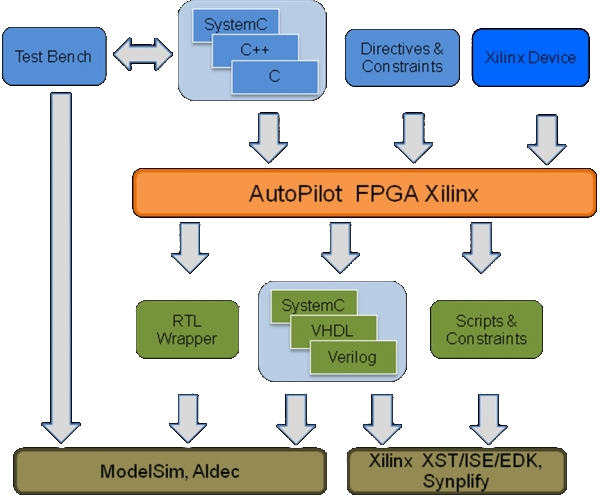
\includegraphics[height=0.88\textheight]{xilinx/autoesl-flow}
    }
\end{frame}

\end{document}